\documentclass[a4paper,12pt]{report}

% Packages for formatting
\usepackage{graphicx} % For including images (e.g., logos)
\usepackage{setspace} % For adjusting spacing
\usepackage{hyperref} % For clickable links
\usepackage{float} % For positioning figures

% Custom title page
\begin{document}

\begin{titlepage}
    \centering
    \vspace*{2cm} % Adjusts vertical position
    
    % Title of the document
    {\Huge\textbf{Guide de l'encodage lumière}}\\[1.5cm]
    
    % Subtitle or project description
    {\Large\textit{Programmer la Chimp pour un spectacle}}\\[2cm]
    
    % Author's name
    {\Large Adrien Hervé}\\[0.5cm]
    
    % Optional: Company or institution
    {\large\textit{Décibels UTC}}\\[3cm]
    
    % Date
    {\large Septembre 2024 - V1.0}\\[3cm]
    
    % Logo
    
\includegraphics[width=0.5\textwidth]{Logos/logo_decibels.png}
    
    \vfill % Pushes the following text to the bottom of the page
\end{titlepage}

% Table of contents
\renewcommand{\contentsname}{Sommaire} % Renames the table of contents
\newpage
\tableofcontents
\newpage

% Content
\chapter{Introduction}
\label{chap:introduction}

Bonjour cher.e lecteur.trice, et bienvenue dans ce guide de l'encodage lumière.
Ce manuel s'adresse à toute personne souhaitant programmer un spectacle sur la console Infinity Chimp 300.
Quel que soit votre niveau de connaissance, après lecture de ce document, vous devriez avoir toutes les clés pour préparer au mieux la console pour un spectacle.
\newline
\newline
Dans ce guide, nous aborderons les bases de la programmation lumière, toute console confondue.
Nous parlerons des protocoles qui permettent de communiquer avec les projecteurs, du lexique associé aux elements programmables et des bonnes pratiques pour préparer un spectacle.
\newline
Nous aborderons ensuite en détail les étapes à suivre pour programmer sur la console.
\newline
Nous verrons aussi les differents outils à notre disposition pour adapter une programmation déjà réalisée en cas de changement quelconque.
\newline
Enfin, nous présenterons quelques outils utiles dans des situations spécifiques ou moins courantes.
\newline
\newline
Il est important de noter que ce guide est particulièrement destiné aux membres de l'association Décibels de l'UTC,
et ainsi, les exemples seront souvent en lien avec le matériel et les activités de l'association.
Cependant, les informations contenues dans ce guide sont générales et peuvent être utilisées pour tout type de spectacle.
\newline
\newline
Bonne lecture !

\chapter{Généralités}
\section{Contrôler des lumières}
\label{sec:controler_lumieres}

La lumière est un élément essentiel de tout spectacle. C'est elle qui permet de mettre en valeur les artistes, de créer des ambiances et de guider le regard du spectateur.
Elle peut aussi constituer un spectacle à part entière, au même niveau que la musique ou la danse.
\newline
C'est pourquoi il est important de pouvoir contrôler intégralement ce que les projecteurs font. C'est le rôle du régisseur lumière.
\newline
Pour cela, il existe des consoles qui sont spécialisées dans la manipulation de projecteurs. Elles offrent une interface accessible pour contrôler les projecteurs, mais aussi pour les programmer.
\newline
Le protocole le plus largement utilisé pour communiquer avec les projecteurs est le protocole DMX. C'est ce protocole qu'il faut comprendre pour commencer à programmer des lumières.

\section{Le DMX}
\label{sec:dmx}

Le DMX est un protocole de communication standardisé qui permet de contrôler des projecteurs ou divers appareils liés à la lumière.
\newline
Ce protocole est unidirectionnel, c'est-à-dire que les informations ne circulent que dans un sens : de la console vers les projecteurs. En aucun cas la console ne reçoit d'informations des projecteurs.
\newline
\newline
Dans la norme DMX, les informations transitent à travers un câble 5 broches. Cependant, deux des broches ne sont pas utilisées par le DMX. C'est pour cela qu'il est aussi possible de transmettre les informations à travers un câble 3 broches (semblable à un connecteur XLR).
\newline
Le premier conducteur est la masse, le second est le signal, et le troisième est le signal inversé (en opposition de phase). On appelle cette construction un signal "balancé" ou "symétrique". Il permet de réduire les perturbations électromagnétiques accumulées le long du câble.
\newline
\newline
Le signal DMX permet d'envoyer 512 $\times$ 8 bits d'information à une fréquence de 44 Hz.
Chaque information de 8 bits est appelée un "canal". Ainsi, chaque canal peut prendre une valeur entre 0 et 255.
\newline
Historiquement, un projecteur n'avait qu'un seul paramètre à contrôler : son intensité. Ainsi, chaque canal correspondait à un projecteur.
Aujourd'hui, les projecteurs sont plus complexes et peuvent avoir plusieurs paramètres à contrôler. C'est pourquoi un projecteur peut occuper plusieurs canaux.
Chaque projecteur occupe alors une plage de canaux contigus, dont la taille dépend du nombre de paramètres à contrôler. L'emplacement du premier canal de la plage est appelé "adresse" du projecteur.
\newline
Par exemple, supposons que nous disposions de 4 projecteurs qui ont chacun 3 paramètres à contrôler (intensité du rouge, intensité du vert et intensité du bleu). Chaque projecteur occupe donc 3 canaux. Le premier projecteur commence à l'adresse 1, le deuxième à l'adresse 4, le troisième à l'adresse 7, et le quatrième à l'adresse 10.
Le canal 1 contrôle l'intensité du rouge du premier projecteur, le canal 6 contrôle l'intensité du bleu du deuxième projecteur, etc.
\newline
\newline
Il est possible de faire passer le signal DMX sur un câble réseau (Ethernet) en utilisant le protocole Art-Net.
Un seul cable RJ45 peut alors transporter jusqu'à 32 768 univers DMX entre la régie et la scène.
\newline
Il faut alors utiliser un Node qui recoit l'Art-Net et qui le convertir en sorties physiques DMX.
\newline
\newline
Par la suite, nous appelerons \textit{Fixture} un appareil qui peut être contrôlé en DMX (souvent un projecteur).

\section{Les paramètres}
\label{sec:param}

Dans cette section, nous allons détailler les différents paramètres que l'on peut généralement contrôler sur un projecteur.
Un paramètre est souvent associé à un canal unique, mais ce n'est pas toujours le cas. Se référer à la section \ref{sec:fixture_patch} pour plus d'informations.

\subsection{Dimmer}
\label{subsec:param_dimmer}

Le dimmer est le paramètre le plus simple : il correspond à l'intensité lumineuse du projecteur. À 0\%, le projecteur est éteint, et à 100\%, il est à pleine puissance.

\subsection{Shutter}
\label{subsec:param_shutter}

Le shutter correspond à l'obturateur du projecteur. Il permet de bloquer la lumière, ou de laisser passer la lumière. Ce terme est hérité des projecteurs traditionnels, qui possédaient un obturateur mécanique.
Aujourd'hui, le shutter et le dimmer ne contrôlent plus deux éléments distincts : tous deux contrôlent l'intensité lumineuse du projecteur. Là où le dimmer contrôle l'intensité globale, le shutter contrôle la fréquence des effets stroboscopiques (effet de clignotement rapide).

\subsection{Couleur}
\label{subsec:param_couleur}

Il existe deux manières de contrôler la couleur d'un projecteur : en utilisant des filtres de couleur, ou en utilisant des LED de couleur.
\newline
Le premier cas se base sur la synthèse soustractive des couleurs : une lumière blanche est émise par le projecteur, et un filtre de couleur est placé devant la lentille pour ne laisser passer que la couleur souhaitée.
Un projecteur peut posséder une roue de couleur, qui contient plusieurs filtres de couleur. Le projecteur peut alors tourner la roue pour changer de couleur.
Il existe aussi des roues de trichromie : trois roues indépendantes respectivement cyan, magenta et jaune présentent un gradient allant du transparent à la couleur pure. En combinant les trois filtres, on peut obtenir n'importe quelle couleur.
Attention cependant, la trichromie a tendance à faire perdre beaucoup de luminosité au projecteur : un rouge obtenu par trichromie sera moins intense et saturé qu'un rouge obtenu par filtre.
\newline
Le deuxième cas se base sur la synthèse additive des couleurs : le projecteur possède des LED de couleur (rouge, vert, bleu) qui peuvent être allumées plus ou moins intensément pour obtenir n'importe quelle couleur.
On peut aussi trouver des projecteurs avec des LED de couleur ambre, blanc ou bien même UV (parfois appelé "lumière noire").

\subsection{Zoom}
\label{subsec:param_zoom}

Le zoom permet de modifier la largeur du faisceau lumineux.

\subsection{Gobo}
\label{subsec:param_gobo}

Un gobo est un filtre placé devant la lentille du projecteur pour projeter une image. Ces effets sont très intéressants pour projeter des motifs sur diverses surfaces, mais aussi pour donner du volume et de la texture au faisceau lumineux dans le brouillard ou la fumée.
Il existe deux types de gobos : les gobos en métal et les gobos en verre.
\newline
Les gobos en métal sont des disques de métal découpés avec des motifs. Ils coûtent peu cher, mais il présentent deux contraintes : ils ne peuvent pas être colorés, et ne peuvent contenir de zone occultante enclavée (un gobo en métal étant troué, une telle zone ne pourrait pas être maintenue).
\newline
Les gobos en verre sont des disques de verre sur lesquels un motif est imprimé. Ils sont bien plus chers, mais se libèrent de ces contraintes.
\newline
\newline
Les gobos peuvent être fixes ou rotatifs. Les gobos fixes sont simplement placés devant la lentille, tandis que les gobos rotatifs sont montés sur un moteur qui les fait tourner.

\subsection{Prisme}
\label{subsec:param_prisme}

Le prisme est un filtre optique qui permet de décomposer le faisceau lumineux en plusieurs faisceaux. Ils peuvent être rotatifs pour créer des effets de rotation.
Les prismes peuvent être linéaires (les faisceaux sont alignés) ou circulaires (les faisceaux sont disposés en cercle).
\newline
Il est possible de cumuler plusieurs gobos et prismes si les roues sont indépendantes.

\subsection{Focus}
\label{subsec:param_focus}

Le focus permet de régler la netteté de l'image projetée. Il n'est jamais simulé sur les logiciels de simulation 3D, il faut toujours le régler avec le projecteur en vrai.
Le point de focus dépend de plusieurs paramètres : la distance entre le projecteur et la surface de projection, le zoom, la position de la roue de gobo dans la machine, la présence d'un prisme, etc.

\subsection{Frost}
\label{subsec:param_frost}

Le frost est un filtre qui permet de diffuser la lumière. Il est souvent utilisé pour adoucir les ombres, ou pour créer des effets de lumière douce. Lorsqu'il est combiné avec un gobo, il permet de créer des effets de flou.
Certains frosts sont continus, permettant de régler l'intensité de la diffusion, tandis que d'autres sont binaires (on/off).

\subsection{Pan}
\label{subsec:param_pan}

Certains projecteurs sont robotisés et peuvent bouger sur deux axes : pan et tilt. On appelle ces projecteurs des "lyres", "moving heads" en anglais.
Le pan correspond à l'axe horizontal : le projecteur peut tourner de gauche à droite.
L'amplitude du pan est souvent de 540°.

\subsection{Tilt}
\label{subsec:param_tilt}

Le tilt correspond à l'axe vertical : le projecteur peut monter et descendre. Son amplitude est souvent de 270°.

\subsection{Control}
\label{subsec:param_control}

Il existe généralement un paramètre "control" qui permet d'effectuer des réglages spécifiques au projecteur à distance. Cela peut être par exemple le reset du projecteur, le réglage de la vitesse des moteurs, l'allumage ou l'extinction de la lampe, etc.

\subsection{Autres}
\label{subsec:param_autres}

Il existe une multitude d'autres paramètres que l'on peut contrôler sur un projecteur. Tout dépend du modèle du projecteur, de sa complexité, et de ses fonctionnalités.
Par exemple, la Robin MegaPointe de chez Robe permet de contrôler le "hotspot", c'est-à-dire la répartition de l'intensité lumineuse dans le faisceau.
D'autres projecteurs peuvent se réapproprier des paramètres existants pour en faire des paramètres spécifiques : par exemple, l'IVL Photon de Minuit Une utilise le paramètre "gobo" pour contrôler une fonctionnalité exclusive de l'appareil.
\newline
Il est donc important de se référer à la documentation du projecteur pour connaître les paramètres qu'il est possible de contrôler et ses fonctionnalités.

\subsection{Et en DMX ?}
\label{subsec:param_dmx}

Il y a plusieurs manières de contrôler ces paramètres en DMX.
\newline
La plus simple est d'assigner un canal à chaque paramètre. Par exemple, le canal 1 contrôle le dimmer, le canal 2 contrôle le shutter, les canaux 3, 4 et 5 contrôlent respectivement le rouge, le vert et le bleu, un canal contrôle la rotation du gobo, etc.
\newline
Il est aussi possible de regrouper plusieurs paramètres sur un seul canal. Par exemple, le canal 1 contrôle le dimmer si sa valeur est inférieure à 128, et le shutter si sa valeur est supérieure à 128.
\newline
Enfin, pour certains paramètres, un seul canal ne suffit pas. Par exemple le pan : un canal offre 256 valeurs. Or, l'amplitude du pan est de 540°. La résolution angulaire est alors de 540°/256 = 2.1°. C'est peu précis et cela peut être visible à l'oeil nu.
Pour résoudre ce problème, nous encodons le pan sur deux canaux, soit 16 bits. Cela offre 65536 valeurs, soit une résolution angulaire de 540°/65536 = 0.008°. C'est bien plus précis.
\newline
\newline
Tout cela est indiqué dans le manuel du projecteur. Un projecteur peut avoir plusieurs modes de fonctionnement, et donc plusieurs associations DMX-paramètres differentes.


\chapter{Encoder la Chimp}
\label{chap:encoder_la_chimp}

\section{Préparer la console}
\label{sec:preparer_la_console}

Nous partirons d'ici d'un show nouvellement crée. Il est possible de créer un show
depuis l'onglet \textit{Backup}.

\subsection{Configurer les sorties}
\label{subsec:prep_sorties}

Par défaut, les sorties physiques de la console sont activées. Les ports DMX A à D sont associés aux univers 1 à 4.
Si vous utilisez un node ArtNet, il faut bien penser à activer le protocole sur la console (\textit{Setup} $\rightarrow$ \textit{Input / Output} $\rightarrow$ \textit{Enable ArtNet}).
Par ailleurs, il faut bien que la console et le node soient sur le même réseau. Il faut donc regler leurs adresse IP en conséquence (\textit{Setup} $\rightarrow$ \textit{Network Settings}).
\newline
Si vous utilisez un visualisateur comme Capture ou Wysiwyg (qui communique en Art-Net), il faut aussi regler l'adresse IP de l'ordinateur sur lequel tourne le visualisateur.

\subsection{Patch}
\label{subsec:prep_patch}

A présent, il faut ajouter les projecteurs à la console. Pour cela, il faut se rendre dans la fenetre \textit{Setup} $\rightarrow$ \textit{Patch}.
\newline
Appuyez sur \textit{Add Fixture} pour ajouter un projecteur. Vous pouvez ensuite choisir le projecteur et son mode dans la liste des fixtures disponibles (\textit{Add Type from Factory Library}).
Si le projecteur ou le mode n'est pas dans la liste, vous pouvez le créer manuellement, voir section \ref{subsec:fixture_patch}.
\newline
Les sorties d'un gradateur sont généralement patchées comme plusieurs \textit{Generic Dimmer}.
\newline
\newline
Une fois le type séléctionné, vous pouvez entrer le nombre de fixtures de ce type qui sont présentes dans votre installation.
\newline
Vous pouvez maintenant choisir l'univers sur lesquelles vous voulez les mettre, et l'adresse de départ.
Si vos projecteurs sont sur plusieurs univers differents, pas de panique, vous pouvez réajuster l'univers et l'adresse une fois les fixtures ajoutées.
\newline
Avant d'ajouter un autre type de fixture, veillez bien à regler les ID et adresses de chaque fixture déjà ajoutée en suivant ce que vous avez fait dans les sections \ref{subsec:patch_id} et \ref{subsec:patch_adressage}.
\newline
\newline
Vous pouvez ensuite faire de même pour toutes les fixtures de votre installation.
\newline
\newline
\textbf{Exemple}
\newline
\newline
Mon plan de feu comporte deux ponts. Le pont de contre contient 4 Dinos et 4 Modenas qui seront sur l'univers 1.
Le pont de face contient 4 Dinos et 4 Modenas qui seront sur l'univers 2, ainsi que 4 PC1000 branchés sur les prises 1 et 3 du gradateur.
Le gradateur est branché seul sur l'univers 3.
\newline
Mon patch sur la console sera donc le suivant :
\begin{figure}[H]
    \centering
    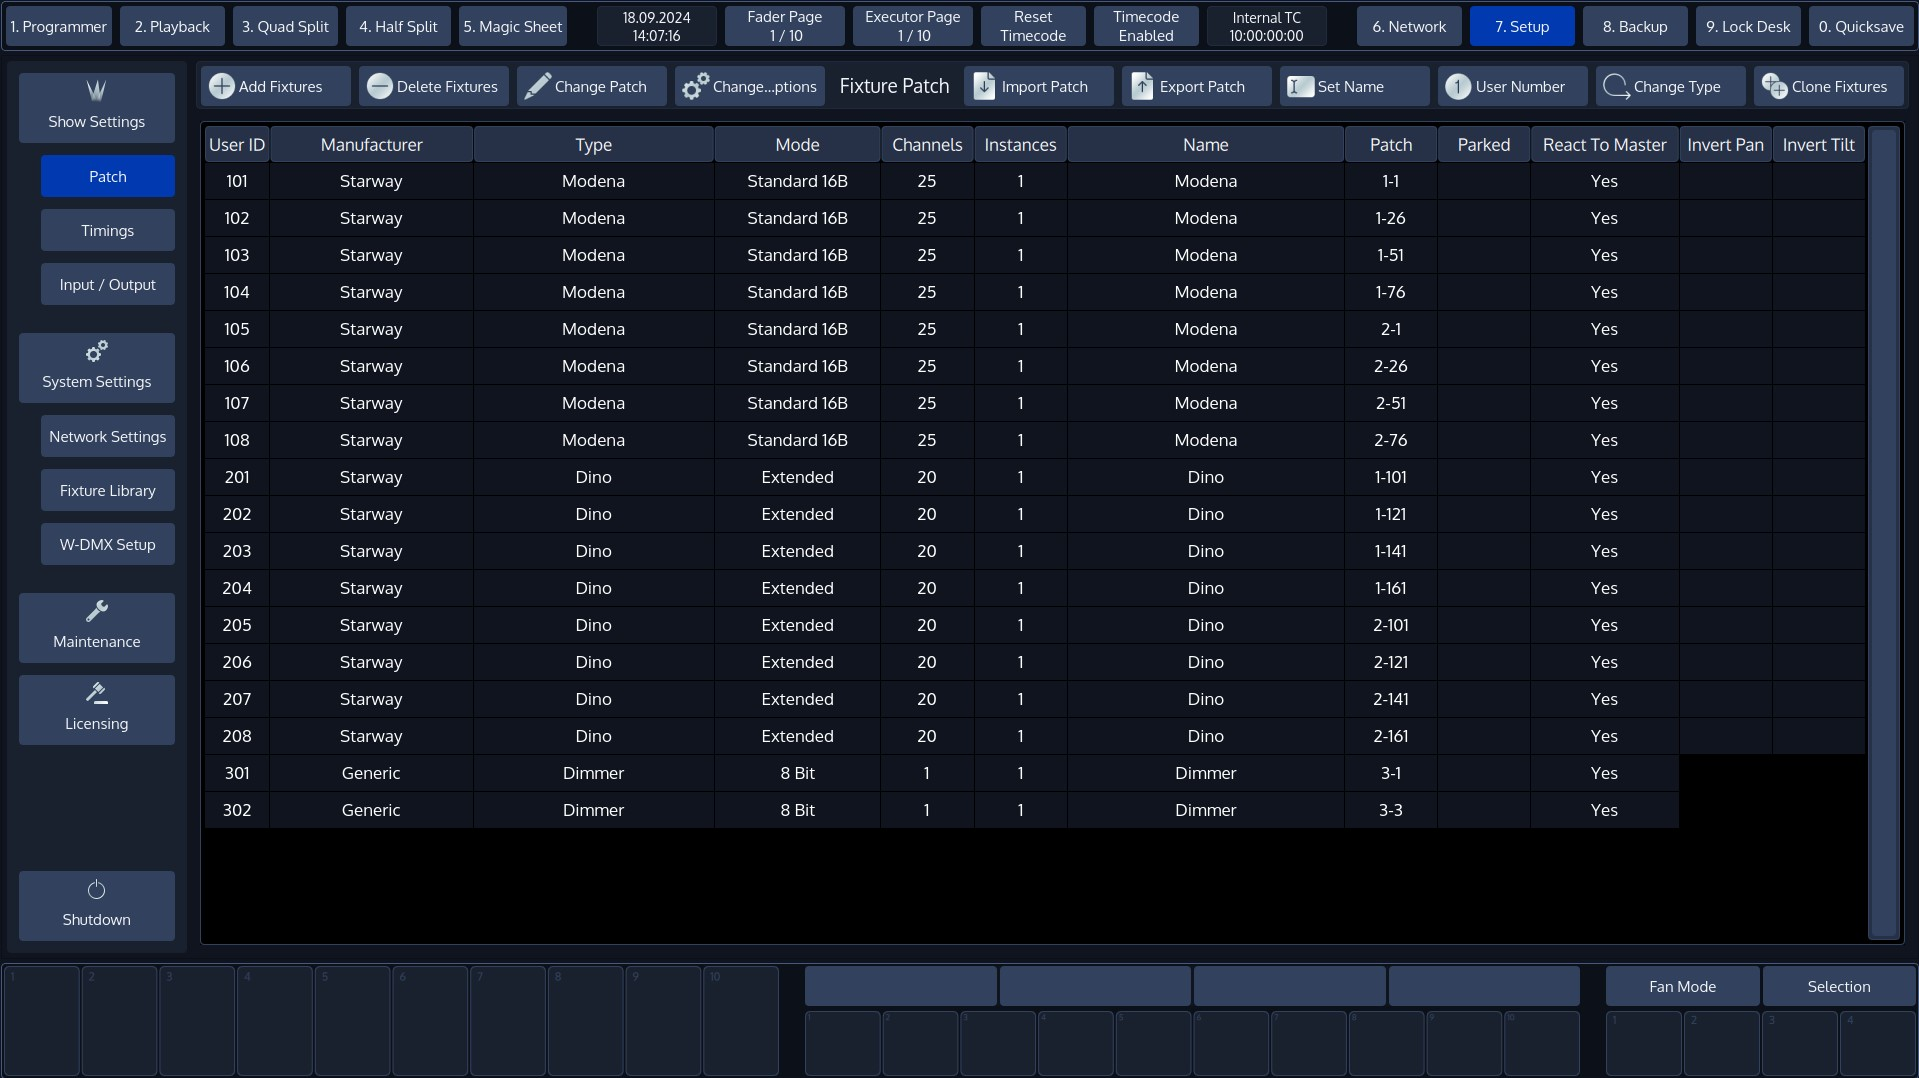
\includegraphics[width=\textwidth]{3 - Encoder la Chimp/Images/patch.jpg}
    \caption{Exemple de patch pour le plan de feu décrit}
    \label{fig:exemple_patch}
\end{figure}

\subsection{Instances}
\label{subsec:prep_instances}

Certaines fixtures, dans certains modes, peuvent comporter plusieurs \textit{instances}. Cela signifie que plusieurs parties d'une même fixture peuvent être contrôlées indépendamment.
\newline
Par exemple, une Modena en mode Pixel16B (69 canaux) comporte 8 instance.
\begin{list}{-}{}
    \item Pan/Tilt, Dimmer général, Zoom, Control, etc.
    \item LED 1 (Couleur, Dimmer et Shutter)
    \item \dots
    \item LED 7 (Couleur, Dimmer et Shutter)
\end{list}

\subsection{Colorer les fixtures}
\label{subsec:prep_colorer}

Pour faciliter la lecture des informations à l'ecran, il peut etre interessant d'associer une couleur à chaque type de fixture.
Par exemple, les Dinos seront en vert, les Modenas en Magenta et les PC1000 en jaune.
\newline
Pour cela, il faut se rendre dans la fenetre \textit{Programmer} et ouvrir une page \textit{Fixtures}.
\newline
Vous pouvez à présent voir toutes vos fixtures. Pour chacune d'entre elles, appuyez deux fois sur la touche \textit{Name} du clavier
et cliquez sur la fixture. Vous pouvez alors choisir une couleur pour cette fixture.
\newline
Par la suite, si vous voulez colorer n'importe quel élément de l'interface, c'est la même manipulation.
\newline
\newline
\textbf{Exemple}
\newline
\newline
Voici le resultat de la coloration pour mon exemple sur la figure suivante :
\begin{figure}[H]
    \centering
    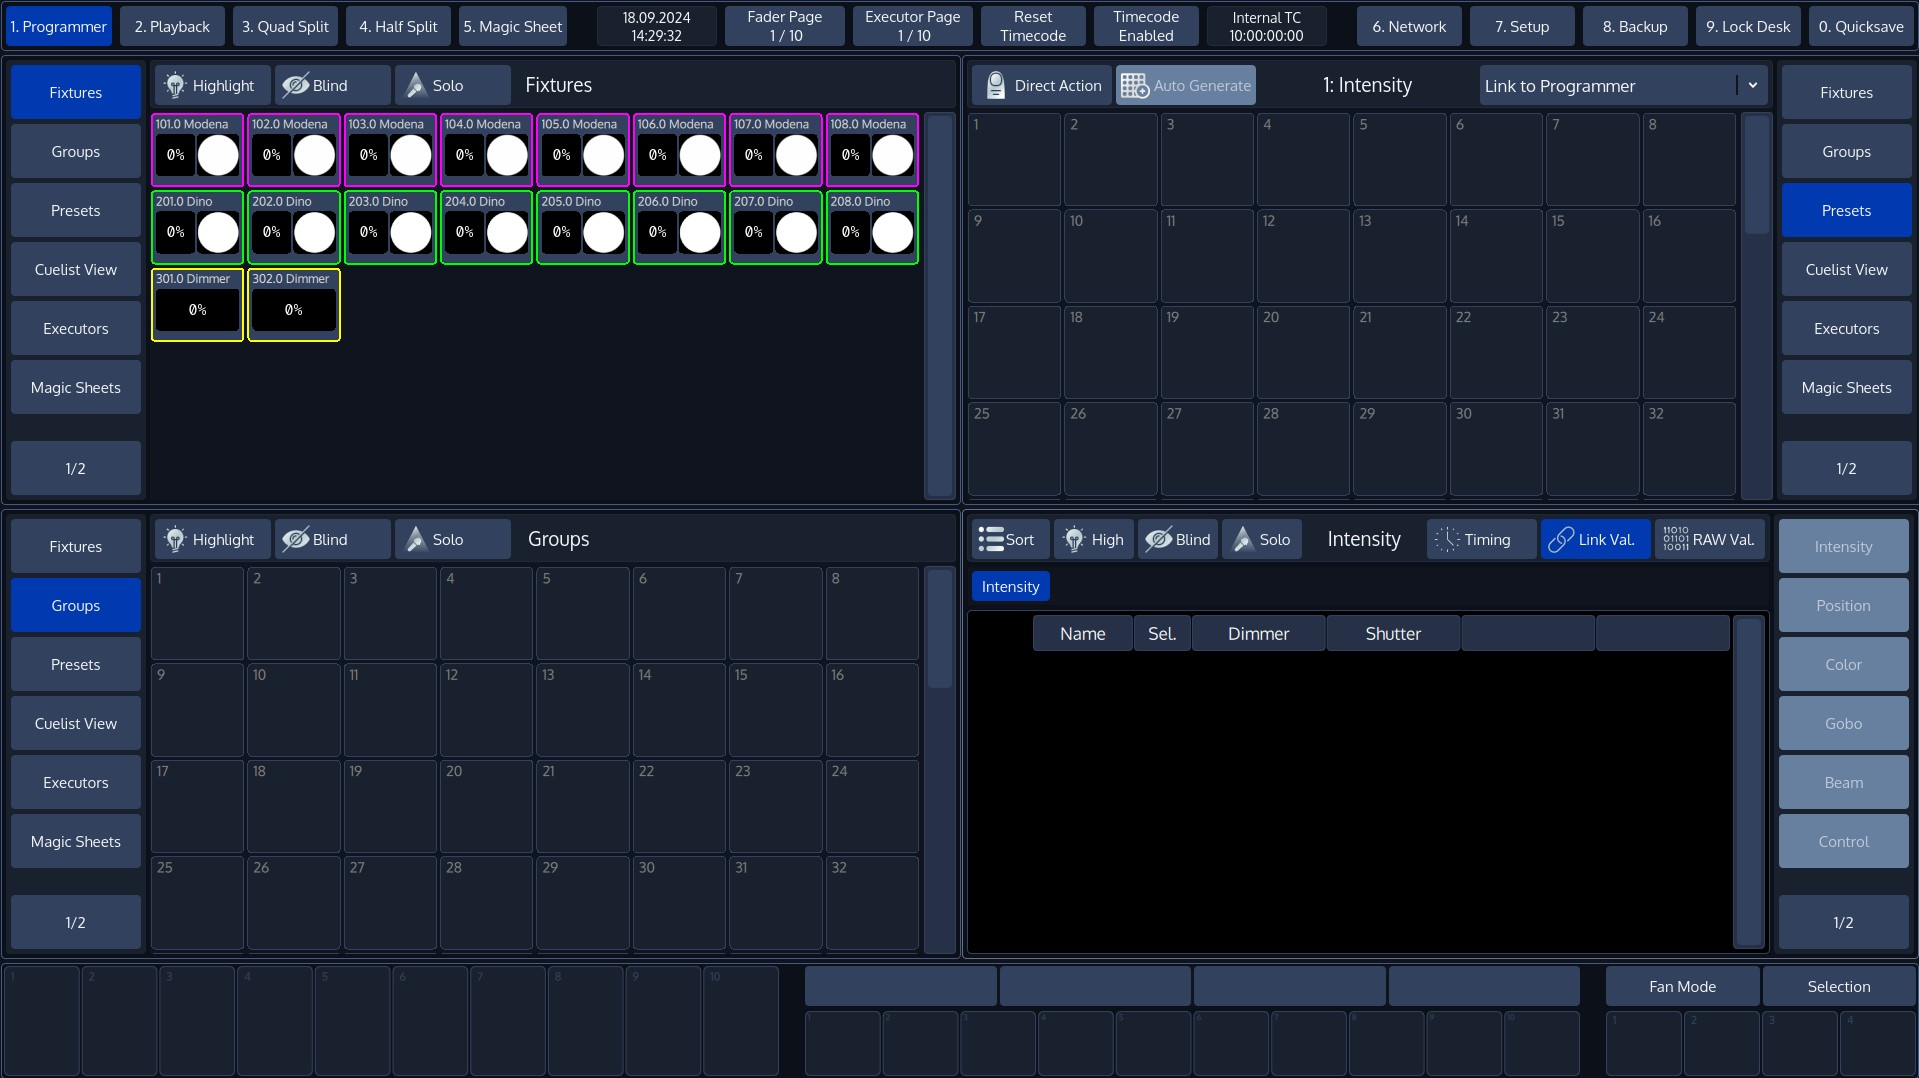
\includegraphics[width=\textwidth]{3 - Encoder la Chimp/Images/fixture_color.jpg}
    \caption{Exemple de coloration des fixtures}
    \label{fig:exemple_color}
\end{figure}

\subsection{Magic Sheet}
\label{subsec:prep_magic_sheet}

La Magic Sheet n'est pas essentielle sur les petites installations, mais elle peut tout de même faire gagner du temps.
Sur les plus grosses scènes, elle est presque indispensable.
\newline
La Magic Sheet est une page personnalisable dans laquelle on peut placer des fixtures ou des groupes de fixtures librement.
\newline
L'idée est alors de faire une page qui représente le plan de feu, avec les fixtures à leur place.
Ainsi, pas besoin de connaitre les ID par coeur pour selectionner une fixture en particulier, is suffir de la chercher dans la Magic Sheet.
\newline
\newline
Pour créer une Magic Sheet, il faut se rendre dans la fenetre \textit{Magic Sheet}, selectionner en haut a droite la page sur laquelle on veut travailler,
et appuyer sur le bouton \textit{Crayon} en haut a gauche.
\newline
On peut ensuite cliquer sur \textit{Add ...} $\rightarrow$ \textit{Fixtures} pour ajouter des fixtures à la page.
\newline
Il est maintenant possible de déplacer les fixtures sur la page.
\newline
\newline
Une fois l'opération, on peut quitter le mode édition en appuyant sur le bouton \textit{Crayon} en haut a gauche.
\newline
En revenant dans le programmer, vous pouvez remplacer la fenetre \textit{Fixtures} par la fenetre \textit{Magic Sheets} pour voir les fixtures à leur place.
\newline
\newline
Pro tip : Pour les fixtures possedant plusieurs instances comme les sunstrip (10!), la Magic Sheet peut vite devenir illisible.
Il donc est possible de regrouper les instances dans un groupe de fixtures (voir section suivante), et de mettre ce groupe dans la Magic Sheet.
\newline
\newline
\textbf{Exemple}
\newline
\newline
Voici un exemple de Magic Sheet pour mon exemple :
\begin{figure}[H]
    \centering
    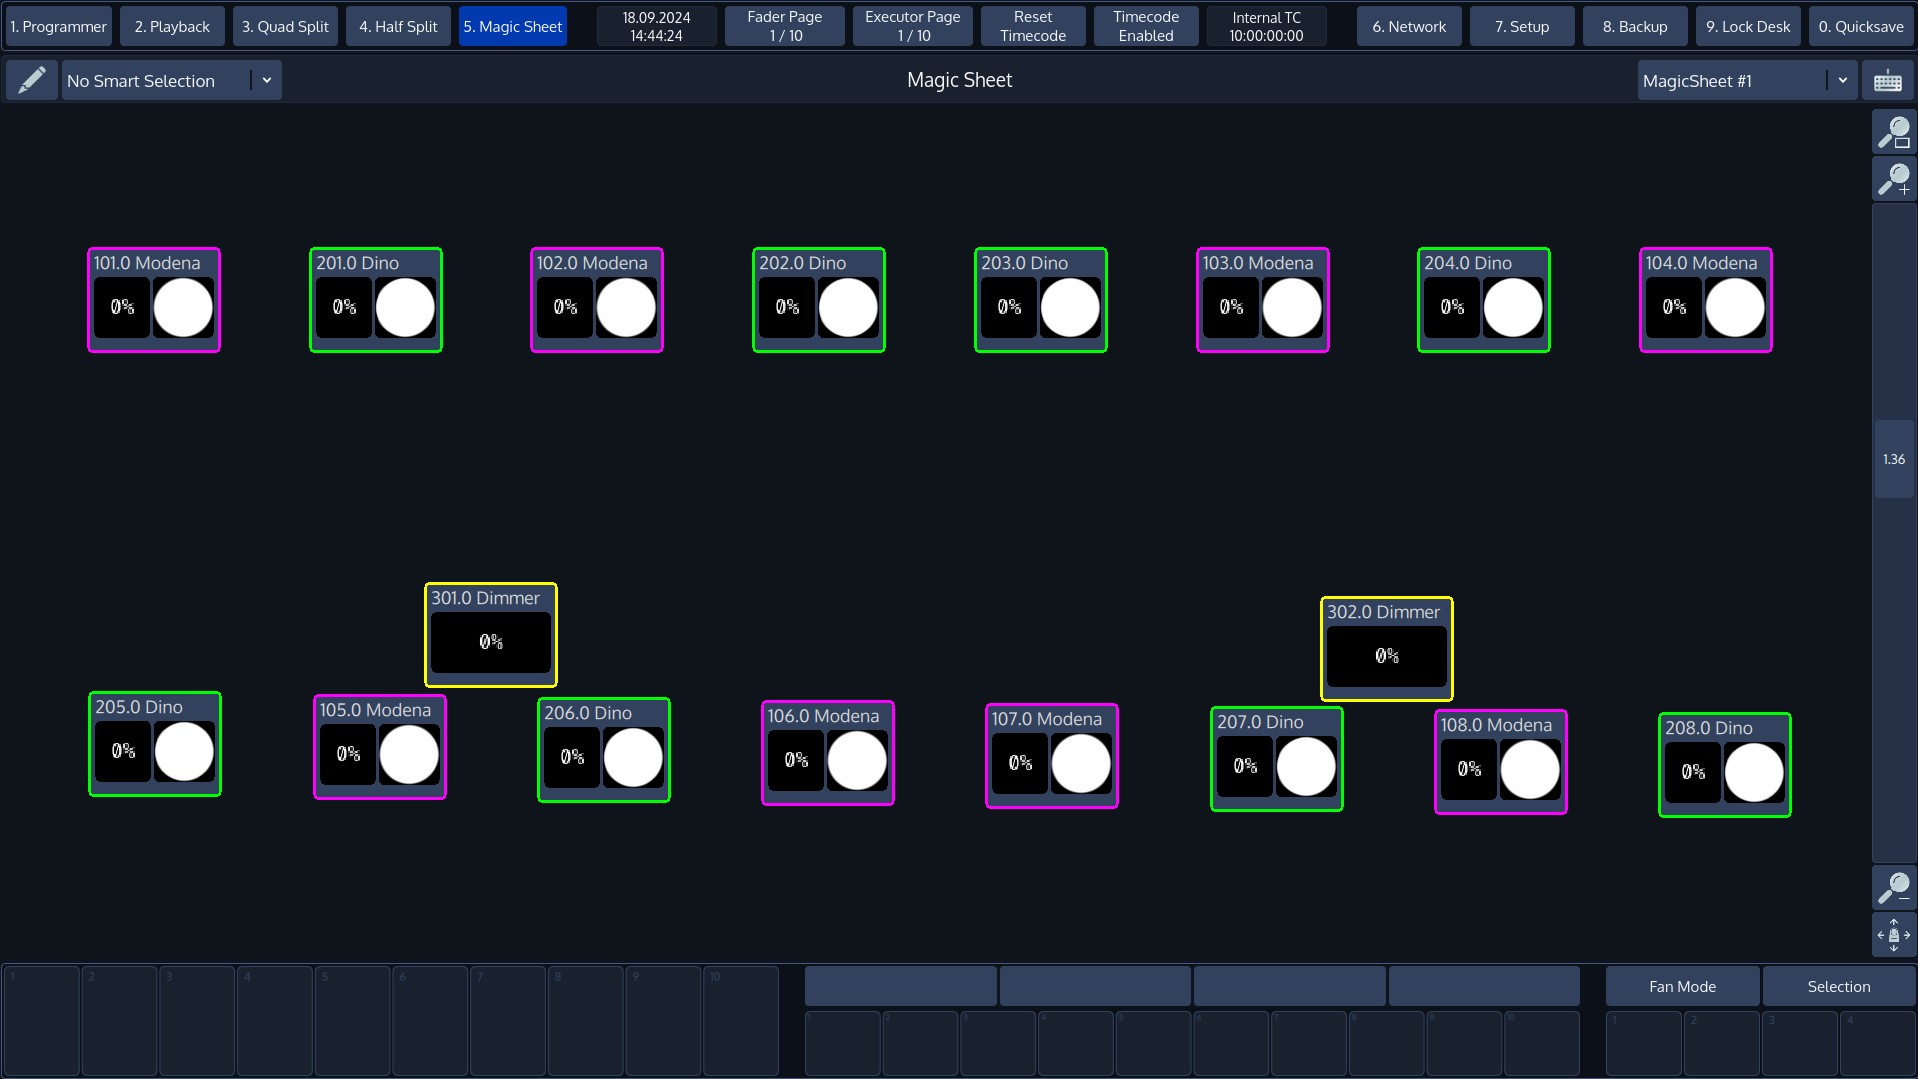
\includegraphics[width=\textwidth]{3 - Encoder la Chimp/Images/magic_sheet.jpg}
    \caption{Exemple de Magic Sheet pour le plan de feu décrit}
    \label{fig:exemple_magic_sheet}
\end{figure}

\subsection{Groupes}
\label{subsec:prep_groupes}

Les groupes permettent de regrouper des fixtures pour les manipuler plus facilement.
\newline
Il est important de noter que les groupes enregistrent l'ordre dans lequel les fixtures ont été selectionnées.
Cela va s'averer important pour la création d'effets (voir section \ref{subsec:prog_effets}).
\newline
\newline
Pour créer un groupe, il faut se rendre dans la fenetre \textit{Programmer} et ouvrir une page \textit{Groups}
(elle est ouverte par defaut dans la fenetre en bas à gauche).
\newline
Selectionnez ensuite les fixtures que vous voulez regrouper dans un ordre interessant (depuis la Magic Sheet ou la page Fixtures), appuyez sur la touche \textit{Rec} du clavier et cliquez sur une case vide de la fenetre de groupe.
Donnez un nom au groupe qui traduit de ce qu'il contient, et l'ordre dans lequel les fixtures ont été selectionnées.
\newline
\newline
\begin{list}{-}{Ordres de selection utiles :}
    \item LTR : Left To Right. Selectionnez les fixtures de gauche à droite, peu importe le pont sur lequel elles sont.
    \item Sym : Symétrique. Selectionnez tantôt une fixture à droite, tantôt une fixture à gauche, en veillant à ne pas selectionner
deux fixtures symétriques. Une fois arrivé à la moitié, selectionnez le symétrique des fixtures déjà selectionnées, dans l'ordre inverse.
\newline
Dans mon exemple, un groupe Sym de Modenas pourrait être : 101, 107, 105, 103, 102, 108, 106 et 104.
    \item D'autres ordres peuvent être interessant, dépendant des effets que vous souhaitez faire.
\end{list}
\textbf{Exemple}
\newline
\newline
Dans mon cas, je vais créer 5 groupes : Modena LTR, Modena Sym, Dino LTR, Dino Sym et PC1000.

\subsection{Grand Master}
\label{subsec:prep_gm}

Pour terminer de préparer la console, il faut créer le Grand Master.
Le Grand Master est un fader qui permet de régler l'intensité générale de tous les projecteurs.
\newline
Pour ce faire, cliquez sur le rectangle associé au premier fader de la console~: il est noté 1 en bas à gauche.
\newline
Allez ensuite dans l'onglet \textit{Global Masters} et selectionnez le \textit{Grandmaster}.
\newline
\newline
Montez le premier fader de la console à 100\% pour que le Grand Master soit à 100\%.
\newline
\newline
\textbf{Exemple}
\newline
\newline
Voici l'état de la console après toutes ces opérations :
\begin{figure}[H]
    \centering
    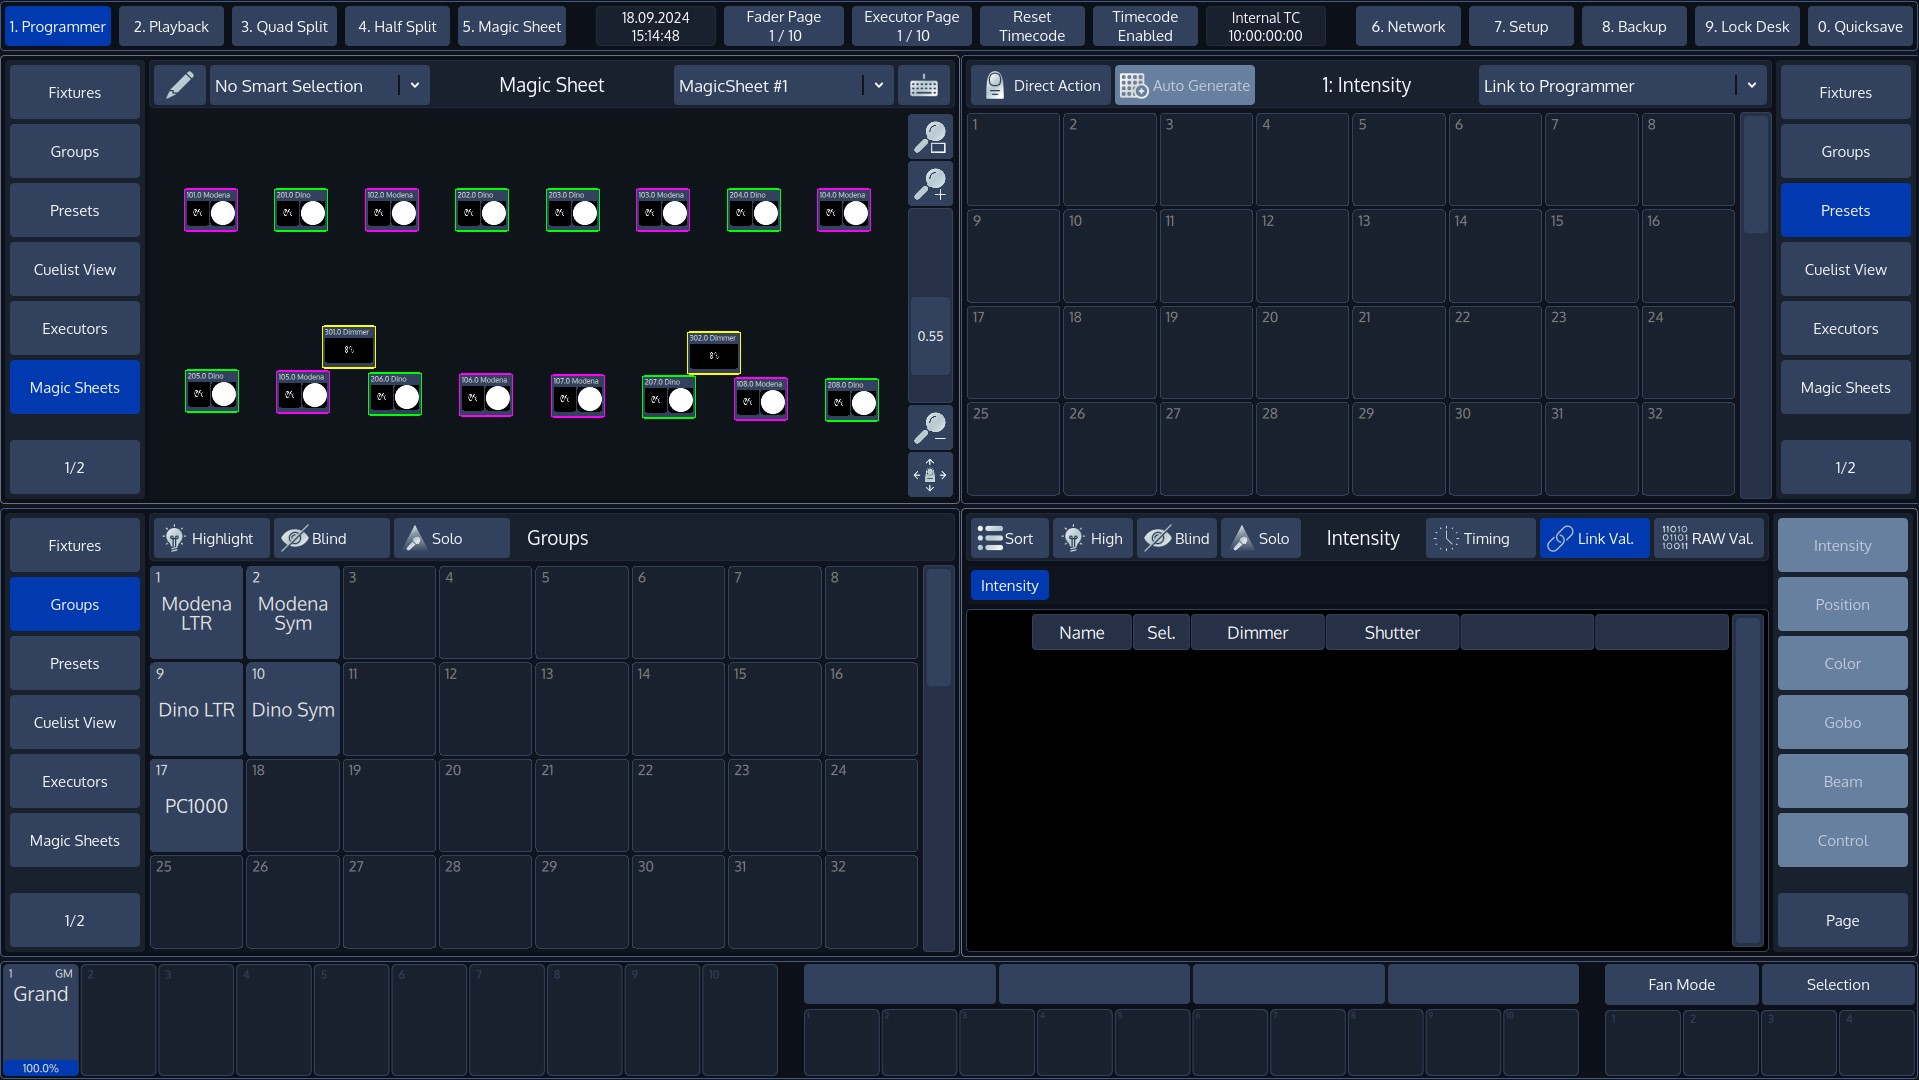
\includegraphics[width=\textwidth]{3 - Encoder la Chimp/Images/prep_final.jpg}
    \caption{Console après préparation}
    \label{fig:prep_finale}
\end{figure}



\end{document}
